\chapter{Alignement de texte}
\label{chap-alignment}
\index{Alignement de texte}
Le principe de l'alignement de texte est simple: quand on aligne deux textes ou plus, le premier est
considéré comme le texte source et les autres comme ses traductions. L'alignement s'effectue au
niveau de la phrase, parce l'alignement au niveau des mots n'est pas encore possible et certainement
pas pertinent. On peut chercher une expression $A$ dans un des textes puis rechercher ses
traductions dans les phrases alignées avec celles contenant $A$.

\bigskip
\noindent Pour ajouter cette fonctionnalité à Unitex, Patrick Watrin a intégré l'outil d'alignement
de texte Open Source \verb+XAlign+, développé au LORIA (\cite{XAlign}). Dans ce chapitre, nous
expliquons comment utiliser le module d'alignement. Le lecteur intéressé par les détails
d'intégration de \verb+XAlign+ peut consulter  \cite{IGML_DumPau08} ou \cite{IGML_PauDum08}, et
\cite{dusko_xalign} pour avoir une idée de ce qui peut être fait avec ce module.

\section{Chargement de textes}
Il faut tout d'abord sélectionner deux textes. Pour cela, allez sur "XAlign>Open files\ldots",
et vous verrez le cadre de la figure \ref{fig-x-text-selection}. Deux formats de textes peuvent être
utilisés: texte brut unicode (comme pour les corpus) ou texte au format TEI
(format de type XML; voir \cite{TEI}). Dans le dernier champ, choisissez un fichier XML
d'alignement, si vous en avez déjà construit un. Si vous choisissez un texte brut, Unitex doit
construire une version TEI de votre texte (pour plus de détails, voir section \ref{section-XMLizer}
au sujet du programme \verb+XMLizer+). Quand vous cliquez sur "OK", le nom d'un fichier  XML vous
est demandé comme le montre la figure \ref{fig-x-tei-name}. Unitex construit alors, si besoin est,
les versions XML de vos textes, et affiche le cadre de la figure \ref{fig-x-frame}. Comme vous
pouvez le constater, chaque texte est représenté sous la forme d'une liste, chaque cellule
comportant une phrase.

\begin{figure}[!ht]
\begin{center}
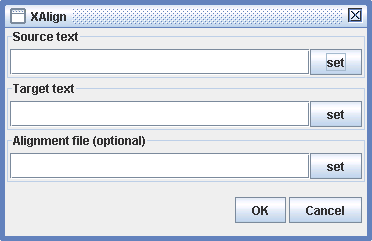
\includegraphics[width=9.5cm]{resources/img/figX-1.png}
\caption{Fenêtre de sélection des textes à aligner\label{fig-x-text-selection}}
\end{center}
\end{figure}

\begin{figure}[!ht]
\begin{center}
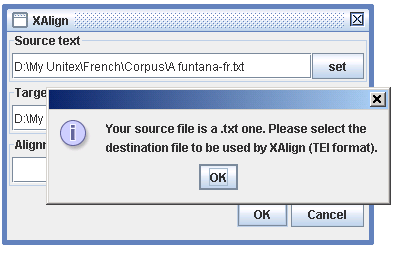
\includegraphics[width=10cm]{resources/img/figX-2.png}
\caption{Attention aux textes bruts\label{fig-x-tei-name}}
\end{center}
\end{figure}
\clearpage

\begin{figure}[!ht]
\begin{center}
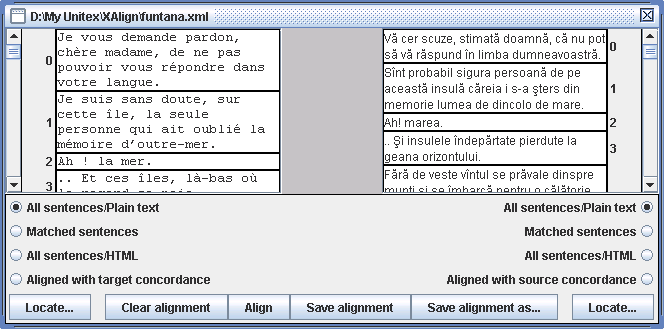
\includegraphics[width=15.5cm]{resources/img/figX-3.png}
\caption{Cadre d'alignement de texte\label{fig-x-frame}}
\end{center}
\end{figure}

\section{Aligner des textes}
Une fois les textes chargés, vous pouvez les aligner en cliquant sur "Align". Le nom du fichier XML
contenant toutes les informations d'alignement vous sera demandé. Ensuite, Unitex lance le programme
\verb+XAlign+, vous visualisez alors l'alignement sous la forme de traits rouges entre les phrases
alignées comme le montre la figure \ref{fig-x-links}.

\begin{figure}[!ht]
\begin{center}
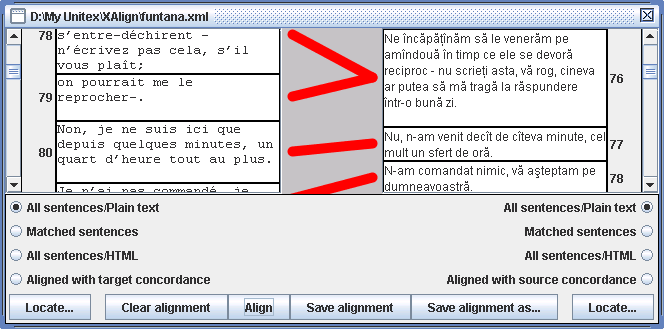
\includegraphics[width=15.5cm]{resources/img/figX-4.png}
\caption{Phrases alignées\label{fig-x-links}}
\end{center}
\end{figure}

\bigskip
\noindent Il est possible d'éditer les liens d'alignement avec la souris. Le fait de cliquer sur un
lien le supprime. Pour ajouter un lien (ou le supprmer, s'il existe déjà), sélectionnez une phrase
avec la souris (dans le texte de votre choix, source ou destination) et déplacez la souris jusqu'à
la phrase correspondante dans l'autre texte. Le lien en cours de création apparaît en jaune comme
le montre la figure \ref{fig-x-adding-a-link}. En le sélectionnant, ce lien est effectivement
ajouté et devient rouge. Une fois toutes les corrections effectuées, sauvegardez le nouvel  
alignement au moyen des boutons "Save alignment" "Save alignment as\ldots".

\begin{figure}[!ht]
\begin{center}
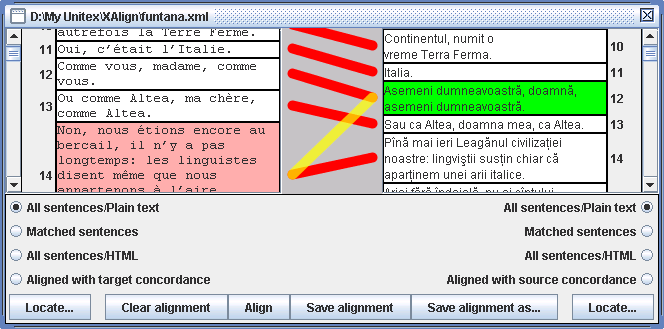
\includegraphics[width=15.5cm]{resources/img/figX-5.png}
\caption{Ajout d'un lien\label{fig-x-adding-a-link}}
\end{center}
\end{figure}

\bigskip
\noindent Une caractéristique intéressante du programme XAlign est qu'il est
\textit{réentrant}.\index{Alignement réentrant} Cela siginifie que vous pouvez utiliser
un alignement existant comme un ensemble de liens obligatoires en tant qu'entrées du processus
d'alignement. Ceci peut-être très utile si vous souhaitez travailler avec des
\textit{mots apparentés}.\index{Mots apparentés} Pour plus de détails au sujet des mots apparentés
 et de XAlign, voir \cite{IGML_PauDum08}.

\clearpage
\section{Recherche de motifs}
Vous pouvez effectuer des recherches de motifs sur chacun des textes, en cliquant sur son bouton
"Locate". La première fois, Unitex vous demandera de construire une version de travail de votre
texte, comme le montre la figure \ref{fig-x-fig6}. Cette version sera prétraitée en tenant compte de
la langue du texte (en particulier, les dictionaires sélectionnés par défaut seront appliqués).

\bigskip
\noindent ATTENTION~: la langue du texte est déterminée à l'aide de son nom complet. Par exemple, 
si votre fichier se trouve dans le répertoire \verb+.../MyUnitex/Klingon/Corpus+, 
la langue considérée sera \verb+Klingon+. Donc, si votre texte n'est pas dans un sous-répertoire
de votre répertoire de travail,\index{Répertoire!personnel de travail} sa langue ne sera pas correctement identifiée.

\begin{figure}[!ht]
\begin{center}
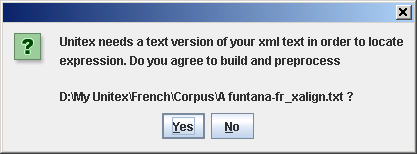
\includegraphics[width=10cm]{resources/img/figX-6.png}
\caption{Unitex doit construire une version de travail du texte\label{fig-x-fig6}}
\end{center}
\end{figure}
 
\begin{figure}[!ht]
\begin{center}
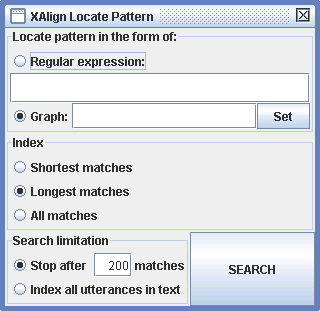
\includegraphics[width=7.8cm]{resources/img/figX-7.png}
\caption{Recherche de motifs sur des textes alignés\label{fig-x-locate-frame}}
\end{center}
\end{figure}

\bigskip
\noindent Une fois qu'Unitex a créé et prétraité la version de travail de votre texte, vous pouvez
effectuer une requête comme indiqué figure \ref{fig-x-locate-frame}. Celle-ci étant faite par le
programme \verb+Locate+,\index{\verb+Locate+} elle est tout à fait semblable à celles effectuées sur
un corpus normal. La seule restriction est qu'il est impossible d'utiliser les sorties des
grammaires si elles en comportent.


\bigskip
\noindent Recherchons par exemple le motif \verb+<manger>+ dans le  texte de notre exemple. Dans un
premier temps, nous n'obtenons aucun résultat, car nous n'avons pas encore changé le mode
d'affichage du texte, qui par  défaut est "All sentences/Plain text". En sélectionnant "Matched
sentences", nous voyons seulement les phrases qui contiennent des occurrences, habituellement
surlignées en bleu comme le montre la figure \ref{fig-x-concord}. En cliquant sur "All
sentences/HTML" nous obtenons toutes les phrases, avec les occurrences surlignées en bleu.

\begin{figure}[!ht]
\begin{center}
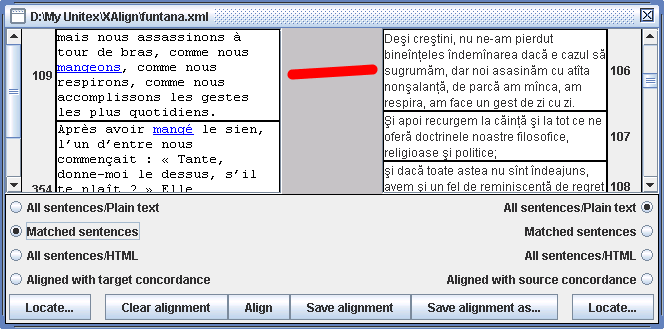
\includegraphics[width=15.5cm]{resources/img/figX-8.png}
\caption{Affichages des phrases reconnues\label{fig-x-concord}}
\end{center}
\end{figure}

\bigskip
\noindent Pour utiliser des textes parallèles, il est intéressant de retrouver les phrases alignées
avec les phrases reconnues. Il suffit pour cela de sélectionner 
\textit{pour l'autre texte}, le mode d'affichage "Aligned with source
concordance". Dans ce mode, Unitex filtre les phrases non liées à des phrases reconnues
dans le texte source. Il est ainsi facile de rechercher une
expression dans un texte et de trouver la phrase correspondante dans l'autre,
comme le montre la figure \ref{fig-x-concord-aligned}.

\begin{figure}[!ht]
\begin{center}
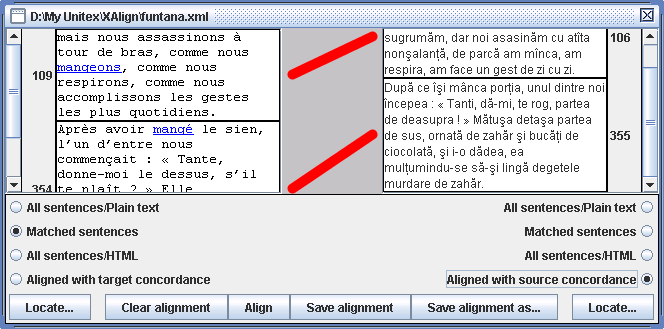
\includegraphics[width=15.5cm]{resources/img/figX-9.png}
\caption{Affichages des phrases reconnues et des phrases auxquelles elles sont liées
\label{fig-x-concord-aligned}}
\end{center}
\end{figure}
